% Version "gros caractères" (grand format, paysage) de la feuille élève
% Série 2. Reprend le même contenu et les mêmes macros que le document
% standard ("Feuille élève - Série 2 - Semaine du 14 au 18 septembre.tex"),
% mais restructuré : une page de garde (titre + liste des automatismes),
% puis un automatisme par page (Vecteurs, A9 Développer factoriser, Algo réparti sur
% 2 pages), puis le tableau réponses réparti sur 2 pages (2 jours par
% page) pour laisser plus de hauteur à chaque ligne. A3/A4 n'ont pas de
% contenu de rappel propre à cette semaine (voir Séquence 1 / Série 1) :
% ils apparaissent dans la liste de la page de garde mais n'ont pas de
% page dédiée.
\documentclass[20pt]{extarticle}
% Latin Modern (vectoriel, toutes tailles) au lieu de Computer Modern
% (tailles Metafont discrètes) : évite les avertissements de substitution
% de taille sur les corps non standards ci-dessous (22pt, 27pt de
% chasse, etc.), qui sinon peuvent légèrement varier -- et donc décaler
% les sauts de page -- selon la distribution LaTeX/l'ordinateur utilisé
% pour compiler.
\usepackage{lmodern}
% extsizes ne fournit pas de size22.clo : on repart de la base 20pt (la plus
% proche disponible) et on surcharge toutes les tailles relatives pour
% qu'elles correspondent à un corps de texte réel de 22pt (rapport 22/20
% appliqué à chaque taille de size20.clo), comme demandé.
\makeatletter
\renewcommand\normalsize{\@setfontsize\normalsize{22pt}{27pt}}
\renewcommand\small{\@setfontsize\small{19pt}{24pt}}
\renewcommand\footnotesize{\@setfontsize\footnotesize{15pt}{19pt}}
\renewcommand\scriptsize{\@setfontsize\scriptsize{13pt}{15pt}}
\renewcommand\tiny{\@setfontsize\tiny{11pt}{12pt}}
\renewcommand\large{\@setfontsize\large{27pt}{33pt}}
\renewcommand\Large{\@setfontsize\Large{33pt}{39pt}}
\renewcommand\LARGE{\@setfontsize\LARGE{39pt}{45pt}}
\renewcommand\huge{\@setfontsize\huge{47pt}{57pt}}
\renewcommand\Huge{\@setfontsize\Huge{57pt}{69pt}}
\makeatother
\normalsize
\usepackage[a4paper,landscape,top=10mm,bottom=10mm,left=12mm,right=12mm]{geometry}
\usepackage[french]{babel}
\usepackage[table]{xcolor}
\usepackage{array}
\usepackage{multirow}
\usepackage{hhline}
\usepackage{pifont}
\usepackage[most]{tcolorbox}
\tcbuselibrary{raster}
\usepackage{ragged2e}
\usepackage{amssymb}
\usepackage{fontawesome5}
\usepackage{enumitem}
\setlist[itemize]{topsep=2pt, itemsep=4pt, parsep=0pt, leftmargin=1.4em, label=$\star$}
\usepackage{bbding}
\usepackage{graphicx}
% Pour insérer le tableau réponses (pages 8-9), compilé à part en A3
% paysage -- geometry interdit de changer le format physique de la page
% en cours de document via \newgeometry, \includepdf est la solution
% standard pour mélanger des formats de page dans un même PDF.
\usepackage{pdfpages}
\usepackage{tikz}
\usetikzlibrary{calc}
\usetikzlibrary{arrows.meta}
% Vrais blocs Scratch 3, mode "impression" (fond blanc, contours et texte
% en noir) pour rester lisible.
\usepackage{scratch3}
\setdefaultscratch{print=true, fill blocks=true, fill gray=1, text color=black}

\pagestyle{empty}
\setlength{\parindent}{0pt}
\renewcommand{\familydefault}{\sfdefault}

% --- Palette (identique au document standard) -------------------------------
\definecolor{inkC}{HTML}{20232B}
\definecolor{inksoftC}{HTML}{565A66}
\definecolor{mutedC}{HTML}{8B8F99}
\definecolor{qcmC}{HTML}{2455B8}
\definecolor{questionC}{HTML}{12805C}
\definecolor{finalC}{HTML}{B5511F}
\definecolor{emptyC}{HTML}{8A909C}
\definecolor{redC}{HTML}{B8342B}
\definecolor{bleuPropriete}{RGB}{41,121,204}
\definecolor{grisExemple}{RGB}{85,85,95}
\definecolor{consoleBgC}{HTML}{1E1E2E}
\definecolor{consoleGreenC}{HTML}{6FCF97}

% Boîte "console" façon terminal.
\newcommand{\consoleBox}[1]{%
  \begin{tcolorbox}[colback=consoleBgC, colframe=consoleBgC, arc=4pt,
    boxrule=0pt, left=10pt, right=10pt, top=4pt, bottom=4pt,
    before skip=0pt, after skip=0pt]
  \ttfamily\color{white}#1
  \end{tcolorbox}%
}
% Panneau générique invisible, pour ranger côte à côte dans un même
% tcbraster des contenus de nature différente en gardant un alignement en
% haut cohérent.
\NewDocumentCommand{\PanelBox}{O{} m}{%
  \begin{tcolorbox}[colback=grisExemple!6, colframe=grisExemple!6, arc=0pt,
    boxrule=0pt, left=3pt, right=3pt, top=0pt, bottom=0pt,
    before skip=0pt, after skip=0pt, #1]
  #2
  \end{tcolorbox}%
}
% Scène Scratch (aperçu) : Tux + bulle de dialogue.
\NewDocumentCommand{\stagePanel}{O{0} m}{%
  \begin{tikzpicture}[baseline=0pt]
    \node[anchor=south west, inner sep=0] (tux) at (0,0)
      {\rotatebox{#1}{
\includegraphics[width=1.7cm]{../assets/img/tux.png}}};
    \node[draw=inkC, fill=white, rounded corners=5pt, line width=1pt,
      align=center, font=\fontsize{10}{12}\selectfont, text width=2.1cm, inner sep=3pt,
      anchor=south west] (bubble) at ([xshift=0.5cm,yshift=1.05cm]tux.south)
      {#2};
  \end{tikzpicture}%
}

\newcommand{\Vj}[1]{\overrightarrow{\text{#1}}}

% Case active du tableau réponses : numéro de question entouré en haut à
% gauche de la case.
\newcommand{\qcase}[1]{%
  \begin{tikzpicture}[baseline=0pt]
    \useasboundingbox (0,0) rectangle (3.65cm,2.9cm);
    \node[anchor=west, circle, draw=inkC, line width=1pt,
          inner sep=2pt, minimum size=1.7em, font=\LARGE, text=inkC]
      at (0.1cm,1.45cm) {#1};
  \end{tikzpicture}%
}
\newcommand{\qempty}{\cellcolor{emptyC}}

% Bandeau de titre (page de garde).
\NewDocumentCommand{\RectoTitre}{m m}{%
  \begin{center}
  \begin{tcolorbox}[
    enhanced,
    width=0.85\linewidth,
    colback=white,
    colframe=inkC,
    boxrule=1.2pt,
    arc=12pt,
    sharp corners=downhill,
    left=16pt, right=16pt, top=26pt, bottom=10pt,
    halign=center,
    overlay={
      \node[fill=white, anchor=west, font=\Large, inner xsep=6pt]
        at ([xshift=20pt]frame.north west) {#1};
    },
  ]
  {\fontsize{48}{52}\selectfont\bfseries #2}
  \end{tcolorbox}
  \end{center}
}

% Carte "automatisme" (engrenage + code + intitulé).
\newcommand{\autoCardLine}[3]{%
  \noindent\tcbox[
    colback=white, colframe=#1, coltext=#1,
    boxrule=1.6pt, arc=7pt, left=14pt, right=14pt, top=4pt, bottom=4pt,
  ]{{\color{#1}\faCogs}~\textcolor{#1}{\LARGE\bfseries #2}~~{\Large\color{inksoftC} #3}}%
  \par
}

% Boîte "À retenir".
\NewDocumentCommand{\ARetenirBox}{O{} m}{%
  \begin{tcolorbox}[
    enhanced, #1,
    colback=bleuPropriete!6, colframe=bleuPropriete,
    boxrule=0pt, arc=0pt, outer arc=0pt,
    left=16pt, right=14pt, top=4pt, bottom=4pt,
    overlay={
      \draw[bleuPropriete, line width=2pt] (frame.north west) -- ++(12pt,0pt);
      \draw[bleuPropriete, line width=2pt] (frame.north west) -- ++(0pt,-12pt);
      \draw[bleuPropriete, line width=2pt] (frame.north east) -- ++(-12pt,0pt);
      \draw[bleuPropriete, line width=2pt] (frame.north east) -- ++(0pt,-12pt);
      \draw[bleuPropriete, line width=2pt] (frame.south west) -- ++(12pt,0pt);
      \draw[bleuPropriete, line width=2pt] (frame.south west) -- ++(0pt,12pt);
      \draw[bleuPropriete, line width=2pt] (frame.south east) -- ++(-12pt,0pt);
      \draw[bleuPropriete, line width=2pt] (frame.south east) -- ++(0pt,12pt);
    },
  ]
    \textbf{\textcolor{bleuPropriete}{À retenir}}\par\vspace{4pt}
    #2
  \end{tcolorbox}%
}
% Boîte "Exemple".
\NewDocumentCommand{\ExempleBoxR}{O{} m}{%
  \begin{tcolorbox}[
    enhanced, #1,
    colback=grisExemple!6, colframe=grisExemple,
    boxrule=0pt, borderline west={3pt}{0pt}{grisExemple},
    arc=0pt, outer arc=0pt,
    left=24pt, right=14pt, top=6pt, bottom=6pt,
    overlay={
      \node[anchor=center, circle, fill=white, draw=grisExemple, line width=1.2pt, minimum size=28pt] at ([yshift=-15pt]frame.north west) {\textcolor{grisExemple}{\fontsize{17}{17}\selectfont\PencilRightUp}};
    },
  ]
    \textbf{\textcolor{grisExemple}{Exemple}}\par\vspace{4pt}
    #2
  \end{tcolorbox}%
}

% Colonnes du tableau réponses.
\newcolumntype{J}{>{\RaggedRight\arraybackslash}m{3.3cm}}
\newcolumntype{N}{>{\centering\arraybackslash}m{3.7cm}}
\newcolumntype{O}{>{\centering\arraybackslash}m{3.85cm}}
\newcolumntype{M}[1]{>{\centering\arraybackslash}m{#1}}

\begin{document}

% ============================ PAGE DE GARDE =================================
\thispagestyle{empty}
\vspace*{0.3cm}
\RectoTitre{Semaine du 14 au 18 septembre}{Automatismes Série 2}

\vspace{0.5cm}

\begin{center}
\begin{minipage}{0.72\linewidth}
\Large
\autoCardLine{qcmC}{A3}{Puissances}
\vspace{7pt}
\autoCardLine{qcmC}{A4}{Écritures d'un nombre}
\vspace{7pt}
\autoCardLine{questionC}{Vecteurs}{Égalité, somme, translations}
\vspace{7pt}
\autoCardLine{qcmC}{A9}{Développer, factoriser}
\vspace{7pt}
\autoCardLine{finalC}{Algo}{}
\end{minipage}
\end{center}

\newpage

% ============================ VECTEURS =======================================
\autoCardLine{questionC}{Translations et vecteurs}{}
\vspace{6pt}
\begin{tcbraster}[raster columns=8, raster column skip=14pt, raster force size=false, raster equal height, raster valign=top, before skip=0pt, after skip=0pt]
\ARetenirBox[raster multicolumn=3]{
  Une \textbf{translation} est une transformation qui permet de faire
  \textbf{glisser} une figure parallèlement à une droite, dans un sens
  donné.\\[4pt]
  \textit{L'image n'est ni retournée, ni déformée}.\\[4pt]
  On peut schématiser ce glissement par une flèche appelée \textbf{vecteur}.
  \vspace{4pt}
  \begin{center}
  \includegraphics[width=5.4cm]{telecabines_schema.pdf}
  \end{center}
}
\ExempleBoxR[raster multicolumn=5]{
  \begin{center}
  \includegraphics[width=0.98\linewidth]{DeLoreanWide.png}
  \end{center}
  \vspace{2pt}
  La figure \textbf{4} est l'image de la figure originale par la translation
  qui transforme A en B.\\[2pt]
  La figure \textbf{2} est l'image de la figure originale par la
  translation de vecteur $\Vj{DC}$.\\[2pt]
  Les figures \textbf{1} et \textbf{3} ne sont pas des images par
  translation~: une translation conserve la taille \emph{et}
  l'orientation.
}
\end{tcbraster}

\newpage

% ====================== CALCUL LITTÉRAL (DISTRIBUTIVITÉ) =====================
\autoCardLine{qcmC}{A9}{Développer, factoriser}
\vspace{3pt}
\ARetenirBox{
  \begin{minipage}[t]{0.47\linewidth}
  \textbf{1. Distributivité simple}\\[4pt]
  Pour tout nombre $k$ et tous nombres $a,b$~:
  \[k(a+b)=k\times a+k\times b\]
  \end{minipage}%
  \hfill
  \begin{minipage}[t]{0.47\linewidth}
  \textbf{2. Double distributivité}\\[4pt]
  Pour tous nombres $a$, $b$, $c$ et $d$~:
  \[(a+b)(c+d)=ac+ad+bc+bd\]
  \end{minipage}
}
\vspace{-20pt}
\ExempleBoxR{
  \begin{minipage}[t]{0.47\linewidth}
  \centering
  \[
  \begin{array}{r@{\,}c@{\,}l}
  A(x) &=& 3(x+5)\\
       &=& 3\times x+3\times5\\
       &=& 3x+15
  \end{array}
  \]
  \vspace{0pt}
  \setlength{\tabcolsep}{4pt}
  {\renewcommand{\arraystretch}{1.1}
  \begin{tabular}{|M{1.3cm}|M{1.3cm}|M{1.3cm}|}
  \hline
  \cellcolor{redC!35} $\times$ & \cellcolor{black!10} $x$ & \cellcolor{black!10} $+5$ \\
  \hline
  \cellcolor{black!10} $3$ & $3x$ & $15$ \\
  \hline
  \end{tabular}}
  \end{minipage}%
  \hfill
  \begin{minipage}[t]{0.47\linewidth}
  \centering
  \[
  \begin{array}{r@{\,}c@{\,}l}
  B(x) &=& (2x-1)(x+4)\\
       &=& 2x^2+8x-x-4\\
       &=& 2x^2+7x-4
  \end{array}
  \]
  \vspace{0pt}
  \setlength{\tabcolsep}{4pt}
  {\renewcommand{\arraystretch}{1.1}
  \begin{tabular}{|M{1.3cm}|M{1.3cm}|M{1.3cm}|}
  \hline
  \cellcolor{redC!35} $\times$ & \cellcolor{black!10} $x$ & \cellcolor{black!10} $+4$ \\
  \hline
  \cellcolor{black!10} $2x$ & $2x^2$ & $8x$ \\
  \hline
  \cellcolor{black!10} $-1$ & $-x$ & $-4$ \\
  \hline
  \end{tabular}}
  \end{minipage}
}

\newpage

% ============================ ALGO (1/2) ======================================
\autoCardLine{finalC}{Algo}{}
\vspace{3pt}
\ARetenirBox{
  Un \textbf{bloc personnalisé} (Scratch) ou une \textbf{fonction} (Python)
  permet de regrouper plusieurs instructions sous un même nom, pour les
  réutiliser en un seul appel.\\[3pt]
  En Python, on la définit avec
  \fbox{\texttt{def nom():}} suivi d'une ligne indentée, puis on l'exécute
  en écrivant dans la console \texttt{nom()}.
}
\vspace{-20pt}
\ExempleBoxR{
\begin{tcbraster}[raster columns=20, raster column skip=10pt, raster force size=false, raster valign=top, before skip=0pt, after skip=0pt]
\PanelBox[raster multicolumn=6]{\centering
  \fontsize{13}{15}\selectfont
  \begin{scratch}[scale=0.72]
    \blockinit{quand \greenflag{} est cliqué}
    \blockmoreblocks{AccordSol}
  \end{scratch}
}
\PanelBox[raster multicolumn=7]{\centering
  \fontsize{13}{15}\selectfont
  \begin{scratch}[scale=0.68]
    \initmoreblocks{définir \namemoreblocks{AccordSol}}
    \blocklook{dire \ovalnum{Sol}}
    \blocklook{dire \ovalnum{Si}}
    \blocklook{dire \ovalnum{Ré}}
  \end{scratch}
}
\PanelBox[raster multicolumn=7]{\centering\stagePanel{Sol, Si, Ré}}
\end{tcbraster}
\vspace{0pt}
\PanelBox{%
  \ttfamily\normalsize
  def AccordSol():\\
  \hspace*{1em}return "Sol", "Si", "Ré"\\[3pt]
  \consoleBox{{\color{consoleGreenC}>>>} AccordSol()\\[3pt]\textbf{('Sol', 'Si', 'Ré')}}
}
}

\newpage

% ============================ ALGO (2/2) ======================================
\autoCardLine{finalC}{Algo}{}
\vspace{3pt}
\ARetenirBox{
  Parfois, un bloc a besoin d'une information précise pour exécuter son
  code~: c'est un \textbf{paramètre}.\\[3pt]
  En Python, on l'écrit entre parenthèses~:
  \fbox{\texttt{def nom(param):}}~; l'appel \texttt{nom(valeur\_voulue)}
  dans la console remplace \texttt{param} par \texttt{valeur} dans le code
  exécuté.
}
\vspace{0pt}
\ExempleBoxR{
\begin{tcbraster}[raster columns=20, raster column skip=10pt, raster force size=false, raster valign=top, before skip=0pt, after skip=0pt]
\PanelBox[raster multicolumn=5]{\centering
  \fontsize{13}{15}\selectfont
  \begin{scratch}[scale=0.6]
    \blockinit{quand \greenflag{} est cliqué}
    \blockmoreblocks{sayHello \ovalnum{John}}
  \end{scratch}
}
\PanelBox[raster multicolumn=9]{\centering
  \fontsize{13}{15}\selectfont
  \begin{scratch}[scale=0.4]
    \initmoreblocks{définir \namemoreblocks{sayHello \ovalmoreblocks{person}}}
    \blocklook{dire \ovaloperator{regrouper \ovalnum{Hello } et \ovaloperator{regrouper \ovalmoreblocks{person} et \ovalnum{!}}}}
  \end{scratch}
}
\PanelBox[raster multicolumn=6]{\centering\stagePanel{Hello John!}}
\end{tcbraster}
\vspace{0pt}
\PanelBox{%
  \ttfamily\normalsize
  def sayHello(person):\\
  \hspace*{1em}return "Hello " + person + "!"\\[3pt]
  \consoleBox{{\color{consoleGreenC}>>>} sayHello("John")\\[3pt]\textbf{'Hello John!'}}
}
}

% ======================= TABLEAU RÉPONSES (pages 8-9, A3 paysage) ============
% Composé et compilé séparément (mêmes contenu/macros, colonnes et cases
% agrandies pour remplir la page) dans
% "Feuille élève - Série 2 - Réponses A3.tex" -- recompiler ce fichier
% avant celui-ci si le tableau réponses change.
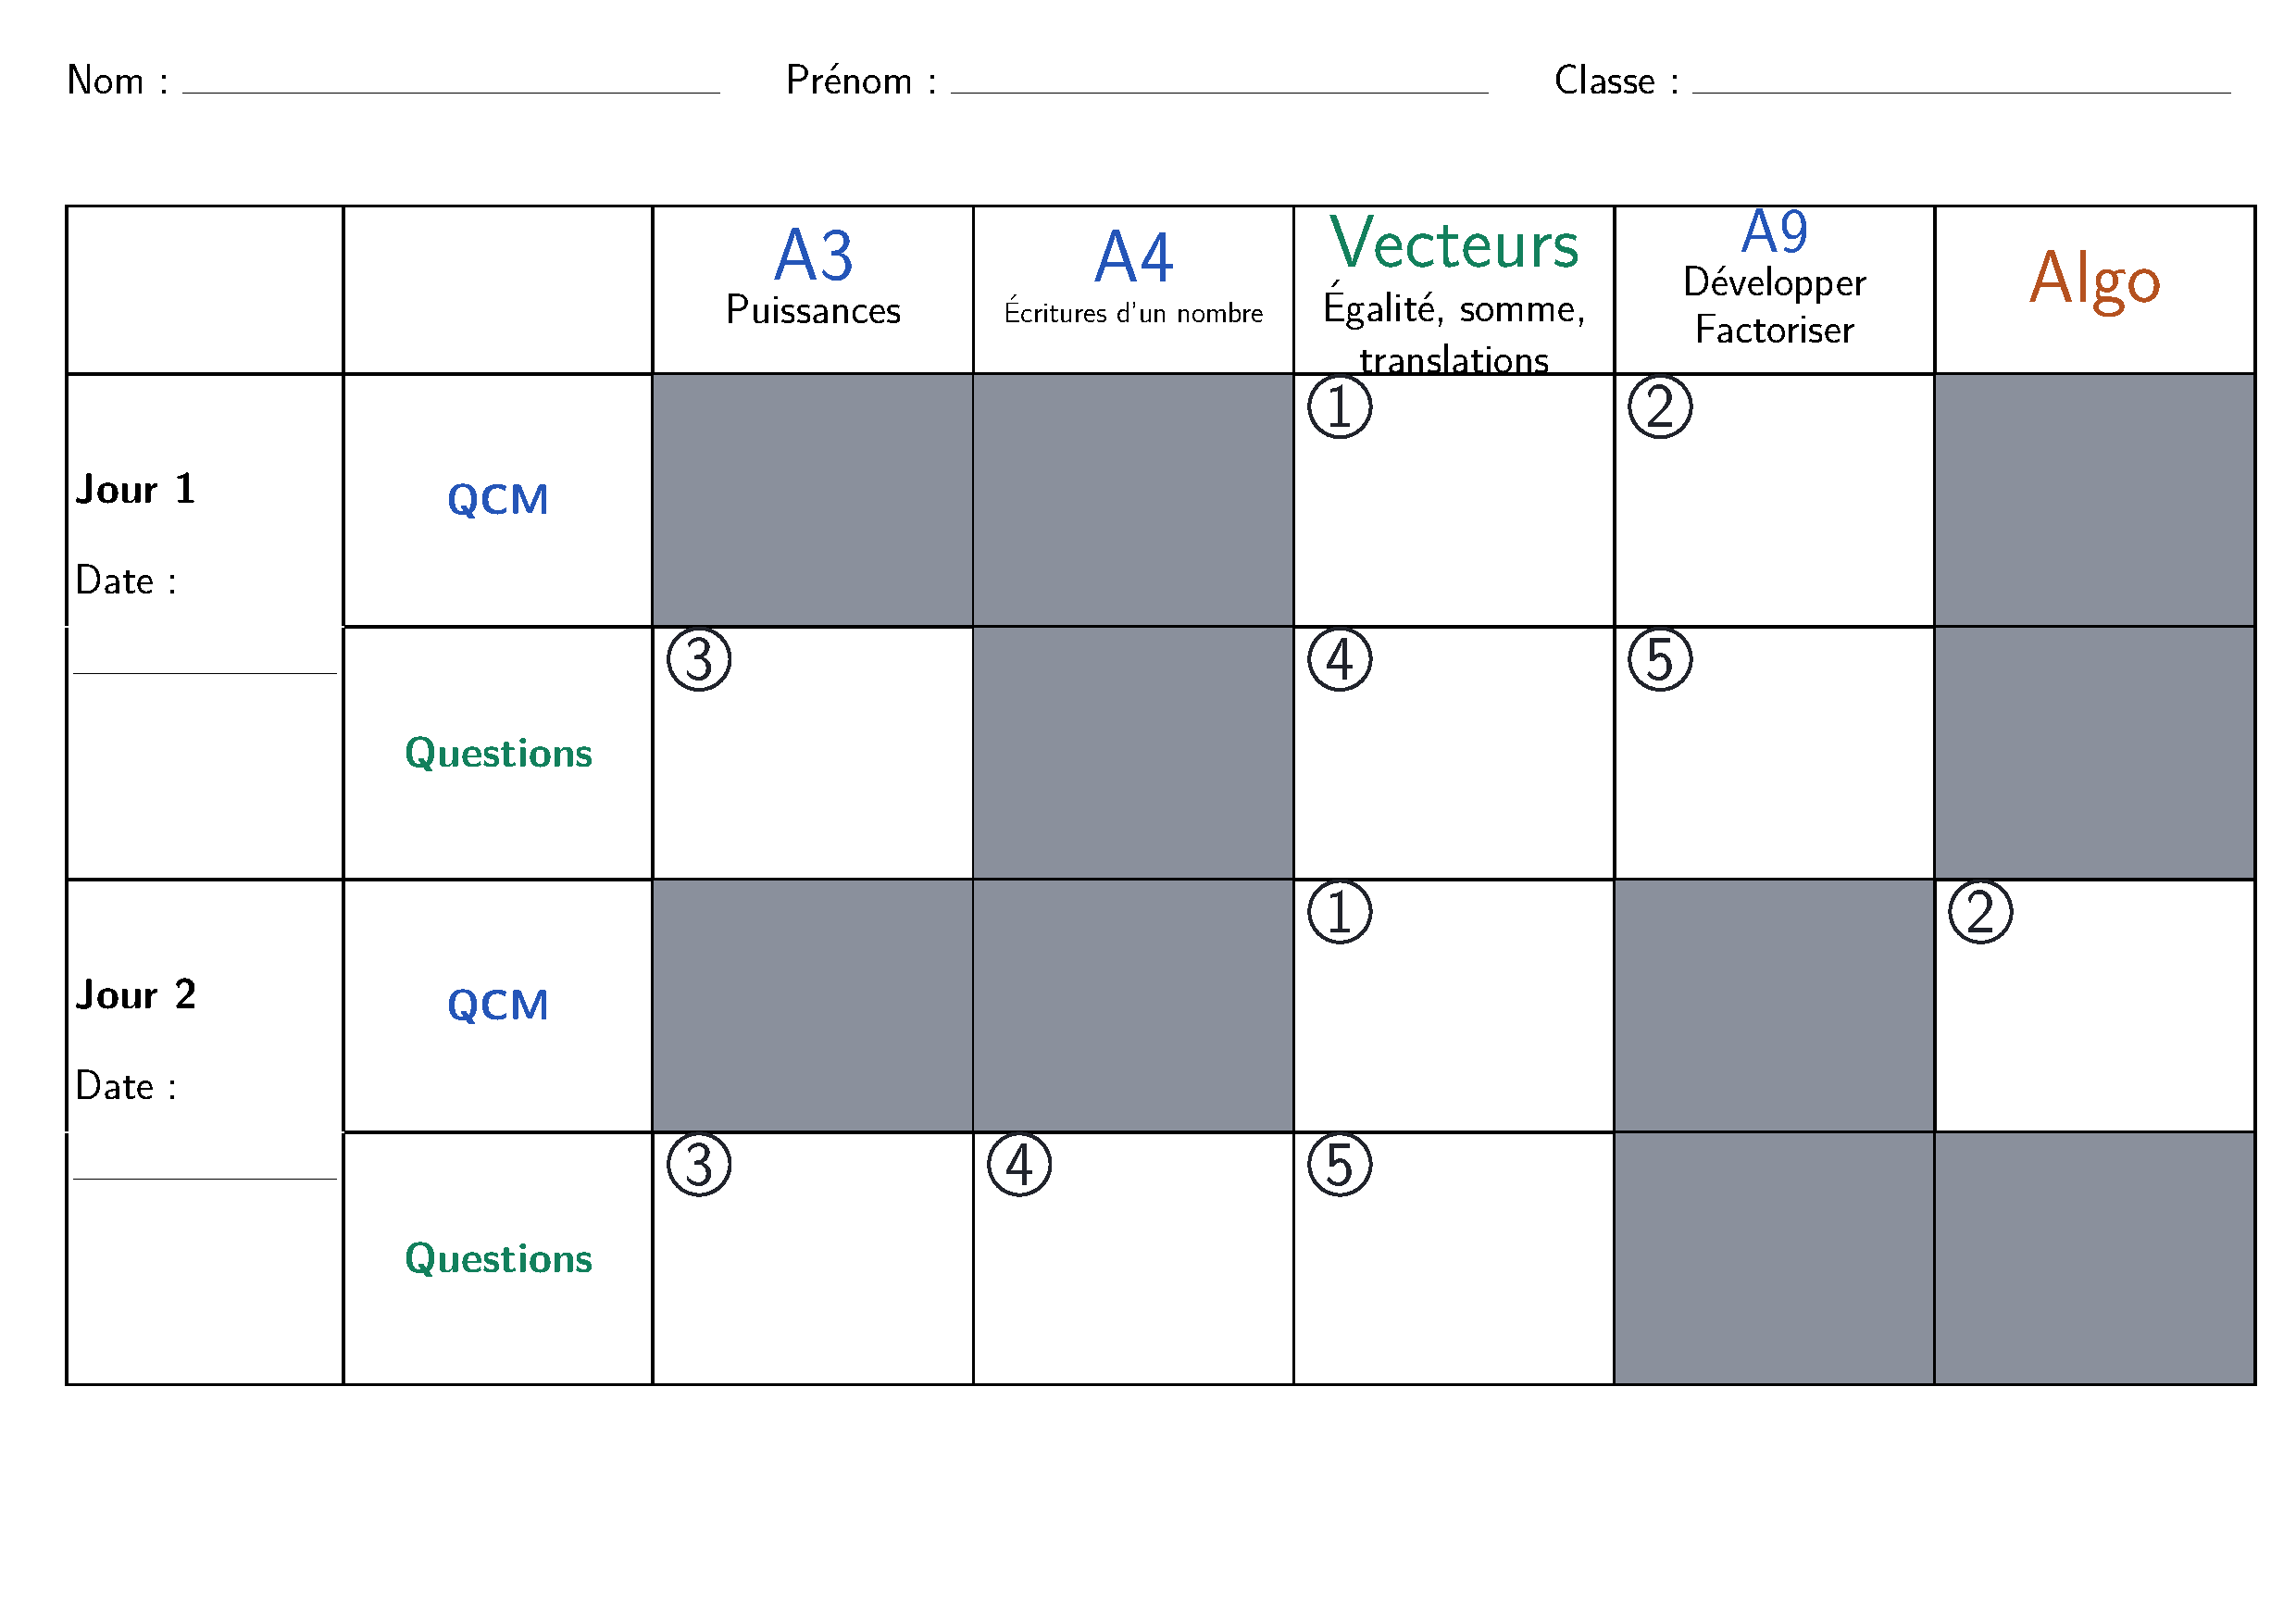
\includepdf[pages=-,fitpaper=true]{Feuille élève - Série 2 - Réponses A3.pdf}

\end{document}
